\chapter{Realizacja projektu}
\label{ch:realizacja_projektu}

Opracowywanie programu w~przypadku korzystania z~Unity jest częściowo podzielone między warstwę kodu a~warstwę projektową,
która obejmuje zarządzanie zasobami, scenami, prefabami oraz innymi elementami, które nie są bezpośrednio związane z~kodem.
Natomiast obie są ze sobą ściśle powiązane, kod definiuje komponenty i~ich zachowanie,
podczas gdy w~edytorze należy je odpowiednio skonfigurować, aby działały zgodnie z~założeniami.
W~związku z~tym przy opisie każdej części aplikacji należy uwzględnić zarówno aspekty kodowe, jak~i~projektowe.\\
\indent Zwracając uwagę na architekturę programu, z~najistotniejszych elementów do zaprojektowania można wyróżnić:

\begin{citemize}
    \item System zarządzania warstwami, rysowaniem ich oraz przechowywaniem informacji o nich,
    \item Narzędzia do rysowania i~edycji, oraz zarządzanie nimi
    \item System zarządzania progresem gry, a~przede wszystkim algorytm weryfikujący poprawność schematów,
    \item Interfejs graficzny pozwalający na interakcję użytkownika z~programem, wybór warstw oraz narzędzi.
\end{citemize}

\section{Warstwy oraz ich rysowanie}
\label{sec:warstwy_oraz_ich_rysowanie}

Ponieważ warstwy, oraz ich rysowanie są kluczowymi elementami, definiującymi działanie reszty programu,
a zarazem stanowią najbardziej obciążającą komputer część projektu,
należało rozpatrzyć najoptymalniejsze rozwiązania do zaimplementowania.
Podstawowym założeniem jest przedstawienie komórki na schemacie jako \textit{GameObject} zawierający dwuwymiarowe,
kwadratowe sprite'y,
stąd cały obszar roboczy jest przedstawiony jako siatka.
W związku z tym najprostszy sposób do zapisania danych warstwy to tablica dwuwymiarowa,
gdzie każdy element tablicy odpowiada jednemu kwadratowi na siatce.
%Jeszcze lepiej podzielić taką tablicę na kilka mniejszych oraz przenieść ją do jednego wymiaru.
Dodatkowo w celu optymalizacji taką tablicę można podzielić na kilka mniejszych,
odpowiedzialnych za różne obszary, a także zamienić je na tablice jednowymiarowe.
Rozwiązanie takie pozwala na optymalniejsze zarządzanie pamięcią,
ponieważ całą warstwę można zapisać jako tablice bitów,
gdzie każdy bit odpowiada jednej komórce i \texttt{1} oznacza,
że jest zajęta a~\textt{0} -- wolna.
W połączeniu z tym rozwiązaniem można wykorzystać dwie metody rysowania warstw:

\begin{citemize}
    \item Rysowanie co modyfikację całej warstwy od nowa -- w tej metodzie cała warstwa jest rysowana od nowa po każdej modyfikacji,
    nie ma potrzeby sprawdzania każdego kwadratu czy jest zajęty, oraz pozwala na pośrednie modyfikowanie narysowanej warstwy,
    bez potrzeby posiadania referencji do obiektów na scenie.
    Wadą jest jednak rysowanie całej warstwy po każdej modyfikacji,
    co przy dużym obszarze roboczym i dużej ilości już narysowanych elementów wpłynie negatywnie na optymalizację.
    \item Rysowanie tylko zmienionych kwadratów -- w tej metodzie komórki są rysowane tylko wtedy, gdy są puste,
    co w ogólnym rozrachunku jest szybsze, jednak wymaga sprawdzania każdej komórki czy nie jest zajęta,
    oraz w celu modyfikacji już istniejących elementów, potrzebne jest posiadanie referencji do GO na scenie.
\end{citemize}

%rysowanie co zmianę całości od nowa, dzięki czemu nie trzeba sprawdzać każdego kwadratu czy już jest zajęty,
%oraz rysowanie tylko zmienionych kwadratów, co w ogólnym rozrachunku jest szybsze,
%natomiast wymaga sprawdzanie każdej komórki czy nie jest zajęta,
%aby nie doszło do sytuacji, gdzie sprite'y się nakładają.
Niestety powyższe rozwiązania wymagają ciągłego iterowania po całej tablicy nawet przy modyfikacji jednego elementu
i albo dodatkowego przetrzymywania referencji, albo ciężkiego obliczeniowo rysowania całej warstwy od nowa.
W związku z tym wybrano inne rozwiązanie, polegające na wykorzystaniu systemu fizyki w silniku Unity,
który pozwala na wykrywanie kolizji pomiędzy obiektami.
Pozwala to na niezależne wykrywanie komórek bez potrzeby referencji do nich,
znacząco upraszczając zarządzanie nimi oraz proces rysowania.
W tym celu do obiektu komórki prócz komponentu \texttt{SpriteRenderer} dodano komponent \texttt{BoxCollider},
dzięki czemu obiekt ten może być wykrywany przez system fizyki.\\
\indent Kolejny sposobem na optymalizację jest wykorzystanie puli obiektów.
Ponieważ w wielu przypadkach potrzebne będzie stworzenie wielu obiektów naraz, co jest kosztowne obliczeniowo,
w trakcie działania programu co klatkę tworzy się ich tylko kilka nieaktywnych, które są następnie przechowywane w puli.
Gdy potrzebny jest nowy obiekt, pobiera się go z puli i aktywuje, a gdy nie jest już potrzebny,
zamiast go usuwać, jest on dezaktywowany i przenoszony z powrotem do puli.
Do implementacji tego mechanizmu dla komórek stworzono komponent \texttt{CellsPool},
posiadający listę struktur \texttt{PoolData} dla każdej z warstw.
Struktura ta przechowuje informację o tym, dla jakiej warstwy jest pula oraz samą pulę obiektów.
Do przetrzymywania tworzonych GO wykorzystano klasę \texttt{Queue},
jest to struktura danych FIFO (ang. \textit{First In, First Out}),
która pozwala na dodawanie elementów na koniec kolejki oraz usuwanie z jej początku.
Aby uporządkować w hierarchii w edytorze wszystkie tworzone w puli obiekty,
jako swojego rodzica mają ustawiony obiekt \texttt{CellsPool}\\
\indent Do definiowania warstw stworzono \texttt{ScriptableObject} \texttt{LayerConfig}.
Zawiera on informacje o nazwie warstwy, jej kolejności na schemacie, jaki sprite ma być rysowany, kolor,
zasady projektowania (minimalna odległość między niesąsiadującymi komórkami, minimalna szerokość)
oraz maksymalną wielkość puli komórek.
Dzięki temu można w łatwy sposób tworzyć nowe warstwy, a także modyfikować definicje już istniejących.
Dodatkowo \texttt{LayerConfig} jest używany jako klucz do identyfikacji warstwy w innych komponentach.
Przykład takiej konfiguracji przedstawiono na rys.~\ref{fig:layer_config}.

\begin{figure}[h]
    \centering
    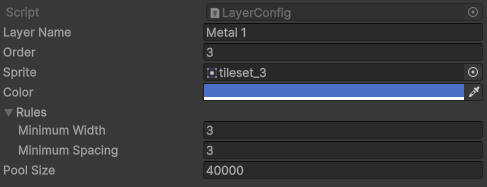
\includegraphics[width=.9\textwidth]{chapters/chapter4/rys/layer_config}
    \caption[Przykładowe okno konfiguracji warstwy \textit{Metal 1}.]
    {Przykładowe okno konfiguracji warstwy \textit{Metal 1}, źródło: opracowanie własne.}
    \label{fig:layer_config}
\end{figure}

%\newpage % TODO: check this if something changes

\indent W trakcie działania programu wszystkie narysowane komórki danej warstwy
są przechowywane w komponencie \texttt{LayerHolder} jako lista obiektów \texttt{GameObject}.
Komponent ten jest także w głównej mierze odpowiedzialny za rysowanie
i usuwanie pojedynczych komórek poprzez metody \texttt{NewCell} oraz \texttt{ReturnCell}.
a także umożliwia dostęp do wszystkich komórek danej warstwy.
Inicjalizacją \texttt{LayerHolder} zajmuje się \texttt{LayersManager}, podczas startu programu.
Z jego głównych funkji można wymienić:

\begin{citemize}
    \item Tworzenie warstw na podstawie konfiguracji z \texttt{LayerConfig},
    \item Przechowywanie referencji do wszystkich warstw,
    \item Wybór oraz zwracanie obecnie rysowanej warstwy,
    \item Włączanie i wyłączanie warstw,
    \item Pośredniczenie przy zwracaniu komórek do puli.
\end{citemize}

Ze względu na istotność tego komponentu, zdecydowano się na zastosowanie wzorca projektowego \textit{Singleton},
dzięki czemu jest on dostępny z każdego miejsca w programie
oraz implikuje posiadanie tylko jednej instancji tego obiektu w trakcie działania programu.
W przypadku Unity, ze względu na to, że klasą bazową komponentów jest \texttt{MonoBehaviour},
należało zaimplementować wzorzec poprzez opracowanie klasy \texttt{MonoSingleton},
której kod przedstawiono na listingu~\ref{lst:monosingleton}.

\begin{lstlisting}[language={C},label=lst:monosingleton,caption={Klasa \texttt{MonoSingleton}}]
public class MonoSingleton<T> : MonoBehaviour where T : Component {
    public static T Instance => _instance;
    private static T _instance;
    protected void Awake() {
        if (_instance != null && _instance != this as T)
            throw new Exception($"Singleton already exists! : {_instance.name}");
        _instance = this as T;
    }
}
\end{lstlisting}

%\newpage
\section{Narzędzia rysowania i edycji}
\label{sec:narzedzia_rysowania_i_edycji}
\section{Sprawdzanie poprawności schematu}
\label{sec:sprawdzanie_poprawnosci_schematu}

Dla każdego poziomu wymagania zapisane są w SO \texttt{Level}, który opisuje,
jakiego rodzaju wymagany jest tranzystor,
między jakimi węzłami powinien się znajdować,
a także jakie są wymagane wymiary bramki.
Przykładowe wymagania dla poziomu 1 przedstawiono na rys.~\ref{fig:level1_requirements}.

\begin{figure}[h]
    \centering
    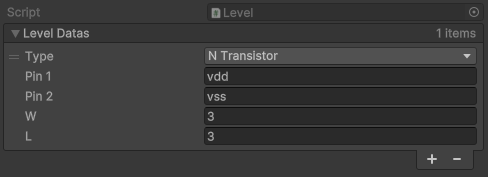
\includegraphics[width=.9\textwidth]{chapters/chapter4/rys/level}
    \caption[Przykładowe wymagania dla poziomu 1.]
    {Przykładowe wymagania dla poziomu 1, źródło: opracowanie własne.}
    \label{fig:level1_requirements}
\end{figure}

Za sprawdzanie poprawności schematu odpowiada komponent \texttt{CheckerManager}, dziedziczący po \texttt{MonoSingleton}.
Zadaniem tego komponentu jest wywołanie skryptu walidującego narysowany schemat,
a następnie porównanie wyników z wymaganiami poziomu.
Na tej podstawie decyduje, czy schemat jest poprawny, czy też nie
i wywołuje okno wyników, które informuje użytkownika o rezultacie.

\subsection{Walidacja schematu}
\label{subsec:walidacja_schematu}

Walidacją schematu zajmuje się komponent \texttt{TopographyValidator}.
Po wywołaniu startu walidacji przez \texttt{CheckerManager},
w pierwszej kolejności wyszukiwane są oznaczenia węzłów, $V_{SS}$ i $V_{DD}$.
Są one punktami zaczepienia dla schematu, a ich brak oznacza błąd.
Gdy znaleziono oba węzły, pobierana jest komórka, jaka znajduje się pod węzłem $V_{DD}$,
przy wykorzystaniu \texttt{Physics.Raycast}.
Komórka ta pełni funkcję punktu startowego w algorytmie znajdywania połączeń.\\
\indent Przed połączeniami, w pierwszej kolejności znajdywane są wszystkie tranzystory na schemacie.
W tym celu z \texttt{LayersManager} pobierane są wszystkie komórki z warstwy \textit{Poly Crystal}.
Dla każdej z komórek sprawdzane jest, 
czy znajduje się pod nią komórka z warstwy \textit{N Diffusion} lub \textit{P Diffusion}.
Do tego celu wykorzystywana jest kolejna funkcja z zasobu systemu fizyki Unity, \texttt{Physics.OverlapBox},
wykrywa ona obiektyw będące w lub stykające się z podanym obszarem.
Jeśli udało się wykryć komórkę z warstw dyfuzyjnych, to znaczy, że znaleziono część tranzystora.
Tworzony jest wtedy nowy obiekt dziedziczący po klasie \texttt{Transistor}, \textt{NTransistor} lub \texttt{PTransistor},
odpowiednio dla tranzystorów nMOS lub pMOS.
W konstruktorze natomiast przekazywane są obecne komórki warstwy polikrystalicznej i dyfuzyjnej.
Obiekt ten ma na celu przechowywanie informacji o tranzystorze oraz wykrycie własnych parametrów.
Po jego utworzeniu wywoływana jest w nim metoda \texttt{FindRest}.
Na podstawie przekazanych wcześniej komórek, ponownie stosując \texttt{Physics.OverlapBox},
znajdywane są sąsiadujące komórki warstw dyfuzyjnej i polikrystalicznej, które się na siebie nakładają.
Aby znaleźć wszystkie komórki, które należą do tranzystora, wykorzystywana jest rekurencja.
Każda znaleziona komórka również próbuje znaleźć sąsiadujące z nią komórki.
Aby uniknąć ponownego wykrycia, komórki po znalezieniu są wyłączane,
dzięki czemu \texttt{Physics.OverlapBox} ich nie wykryje.
Po wyśledzeniu wszystkich komórek, które należą do tranzystora,
w ich miejsce wstawiany jest GO z \texttt{BoxCollider}'em o wymiarach tranzystora,
do których referencje są przechowywane w obiekcie tranzystora.
Dzięki temu znacząco uproszczone będzie wykrycie połączeń z tranzystorami.
Przy ustawianiu rozmiaru komponentu \texttt{BoxCollider}, przy okazji obliczane są wymiary bramki tranzystora,
Główny kod funkcji do znajdywania tranzystorów przedstawiona jest na listingu~\ref{lst:find_transistors}.
Aby uniknąć zawieszenia się pętli programu,
zastosowano przy wyszukiwaniu komórek tranzystora system asynchroniczności \textit{UniTask}.

\begin{lstlisting}[language={C},label=lst:find_transistors,caption={Metoda \texttt{FindTransistors} wyszukjąca tranzystory na schemacie}]
private async UniTask FindTransistors() {
    var polys = LayersManager.Instance.LayerHolders[polyLayer].Cells;
    List<GameObject> usedPolys = new();
    Vector3 overlapSize = new Vector3(0.45f, 0.45f, 0.6f);
    foreach (var poly in polys) {
        if (usedPolys.Contains(poly)) continue;
        var position = poly.transform.position;
        position.x += 0.5f;
        position.y += 0.5f;
        position.z += 0.5f;
        var overlaps = Physics.OverlapBox(position, overlapSize);
        foreach (var overlap in overlaps) {
            if (overlap.gameObject.CompareTag("P Diffusion")) {
                var pTransistor = new PTransistor(poly, overlap.gameObject); 
                await pTransistor.FindRest();
                pTransistor.CreateCollider().Forget();
                usedPolys.AddRange(pTransistor.Polys);
                _pTransistors.Add(pTransistor);
            }
            else if (overlap.gameObject.CompareTag("N Diffusion")) {
                var nTransistor = new NTransistor(poly, overlap.gameObject);
                await nTransistor.FindRest();
                nTransistor.CreateCollider().Forget();
                usedPolys.AddRange(nTransistor.Polys);
                _nTransistors.Add(nTransistor);
            }
        }
    }
    await UniTask.Yield();
    await UniTask.Yield();
}

\end{lstlisting}

Po znalezieniu wszystkich tranzystorów wywoływana jest funkcja \texttt{StartSearch}.
Rozpoczyna ona przeszukiwanie połączeń od komórki pod oznaczeniem $V_{DD}$.
W pierwszej kolejności tworzony jest obiekt węzła \texttt{Node}, oznaczony jako \textit{vdd},
który przechowuje w listach wszystkie znalezione komórki,
kontakty oraz tranzystory typu p i n.
Następnie wywoływana jest metoda \texttt{SearchByOverlap},
której przekazywana jest pozycja startowej komórki oraz obecny węzeł.
Ma ona za zadanie znaleźć wszystkie obiekty sąsiadujące z obecnym,
na podstawie \texttt{Physics.OverlapBox}.
i zapisanie ich do odpowiednich list w obiekcie \texttt{Node}.\\
\indent W przypadku znalezienia tranzystora należy połączyć go z węzłem,
co jest wykonywane przez funkcję \texttt{ConnectTransistor}.
W obiekcie \texttt{Transistor} do wolnego pinu jest przekazywany obecny węzeł,
przy czym zapisywane jest także, po jakiej stronie tranzystora znajduje się ten pin,
jak również to, że drugi wolny pin jest po przeciwnej stronie.\\
\indent Gdy znalezionym obiektem w funkcji \texttt{SearchByOverlap} jest komórka,
dla niej również wywoływana jest ta funkcja, a jako \texttt{Node} przekazywany jest ten obecnie przeszukiwany.
Aby uniknąć ponownego wykrywania, podobnie jak w przypadku tranzystorów,
już wykryte komórki są wyłączane.\\
\indent Gdy znaleziono wszystkie obiekty dla danej warstwy,
w przypadku gdy znaleziono kontakty, ponawia się przeszukiwanie, dla tej warstwy, z którą występuje połączenie.
Natomiast dla każdego ze znalezionych tranzystorów,
tworzony jest nowy węzeł po stronie wolnego pinu tranzystora,
do którego jest też automatycznie podłączany.
Następnie cały proces jest powtarzany dla nowego węzła.
Dla każdej badanej pozycji jest także dodatkowo sprawdzanie, czy nie pokrywa się z oznaczeniem $V_{SS}$.
Jeśli tak, to obecny węzeł jest oznaczany jako \textit{vss}.
Proces znajdywania połączeń jest powtarzany, aż do momentu,
gdy nie będzie już możliwe wykrycie nowych obiektów.
Główną funkcję \texttt{SearchByOverlap} odpowiedzialną za przeszukiwanie przedstawiono na listingu~\ref{lst:search_overlap}.
Ponownie zastosowano tutaj system asynchroniczności \textit{UniTask}.

\begin{lstlisting}[language={C},label=lst:search_overlap,caption={Metoda \texttt{SearchOverlap} wykrywające sąsiadujące obiekty}]
private async UniTask SearchByOverlap(Vector3 center, Node node) {
    center.x += 0.5f;
    center.y += 0.5f;
    var overlaps = Physics.OverlapBox(center, _overlapSize);
    foreach (var overlap in overlaps) {
        if (CheckForVss(overlap.transform.position)) node.ChangeID("vss");
        if (overlap.gameObject.CompareTag("Contact"))  {
            if (node.Contacts.Contains(overlap.gameObject)) continue;
            node.Contacts.Add(overlap.gameObject);
            overlap.gameObject.SetActive(false);
        }
        else if (overlap.gameObject.CompareTag("P Transistor")) {
            var pTransistor = FindPTransistor(overlap.gameObject);
            if (node.PTransistors.Contains(pTransistor)) continue;
            ConnectTransistor(node, pTransistor, overlap.transform.position);
        }
        else if (overlap.gameObject.CompareTag("N Transistor")) {
            var nTransistor = FindNTransistor(overlap.gameObject);
            if (node.NTransistors.Contains(nTransistor)) continue;
            ConnectTransistor(node, nTransistor, overlap.transform.position);
        }
        else {
            var position = overlap.transform.position;
            node.Cells.Add(overlap.gameObject);
            overlap.gameObject.SetActive(false);
            await SearchByOverlap(position, node);
        }
    }
}

\end{lstlisting}

\subsection{Finalizacja sprawdzania}
\label{subsec:finalizacja_sprawdzania}

Po zakończeniu walidacji przez \texttt{TopographyValidator} wywołuje on wydarzenie \texttt{OnValidationEnd},
w którym przekazuje wszystkie wykryte tranzystory, wraz z ich połączeniami i wymiarami.
Iterując po elementach zawartych w wymaganiach poziomu,
porównuje się je z wykrytymi tranzystorami.
Gdy któryś z tranzystorów spełnia jedno z wymagań, jest usuwany z listy wykrytych.
Jeśli pod koniec w liście wykrytych tranzystorów nie ma już żadnych elementów,
to znaczy, że schemat jest poprawny.
Wyświetlane jest wtedy okno informujące o sukcesie.
W przeciwnym wypadku gdy pozostały jeszcze tranzystory, to znaczy, że schemat jest niepoprawny.
\section{Interfejs użytkownika}
\label{sec:interfejs_uzytkownika}

Ostatnim elementem aplikacji,
łączącym wszystkie funkcje w całość oraz umożliwiającym użytkownikowi interakcję z programem,
jest interfejs użytkownika (ang. \textit{User Interface}, UI).
Ostateczny widok okna aplikacji podczas działania programu pokazano na rysunku~\ref{fig:ui_final}.

\begin{figure}[H]
    \centering
    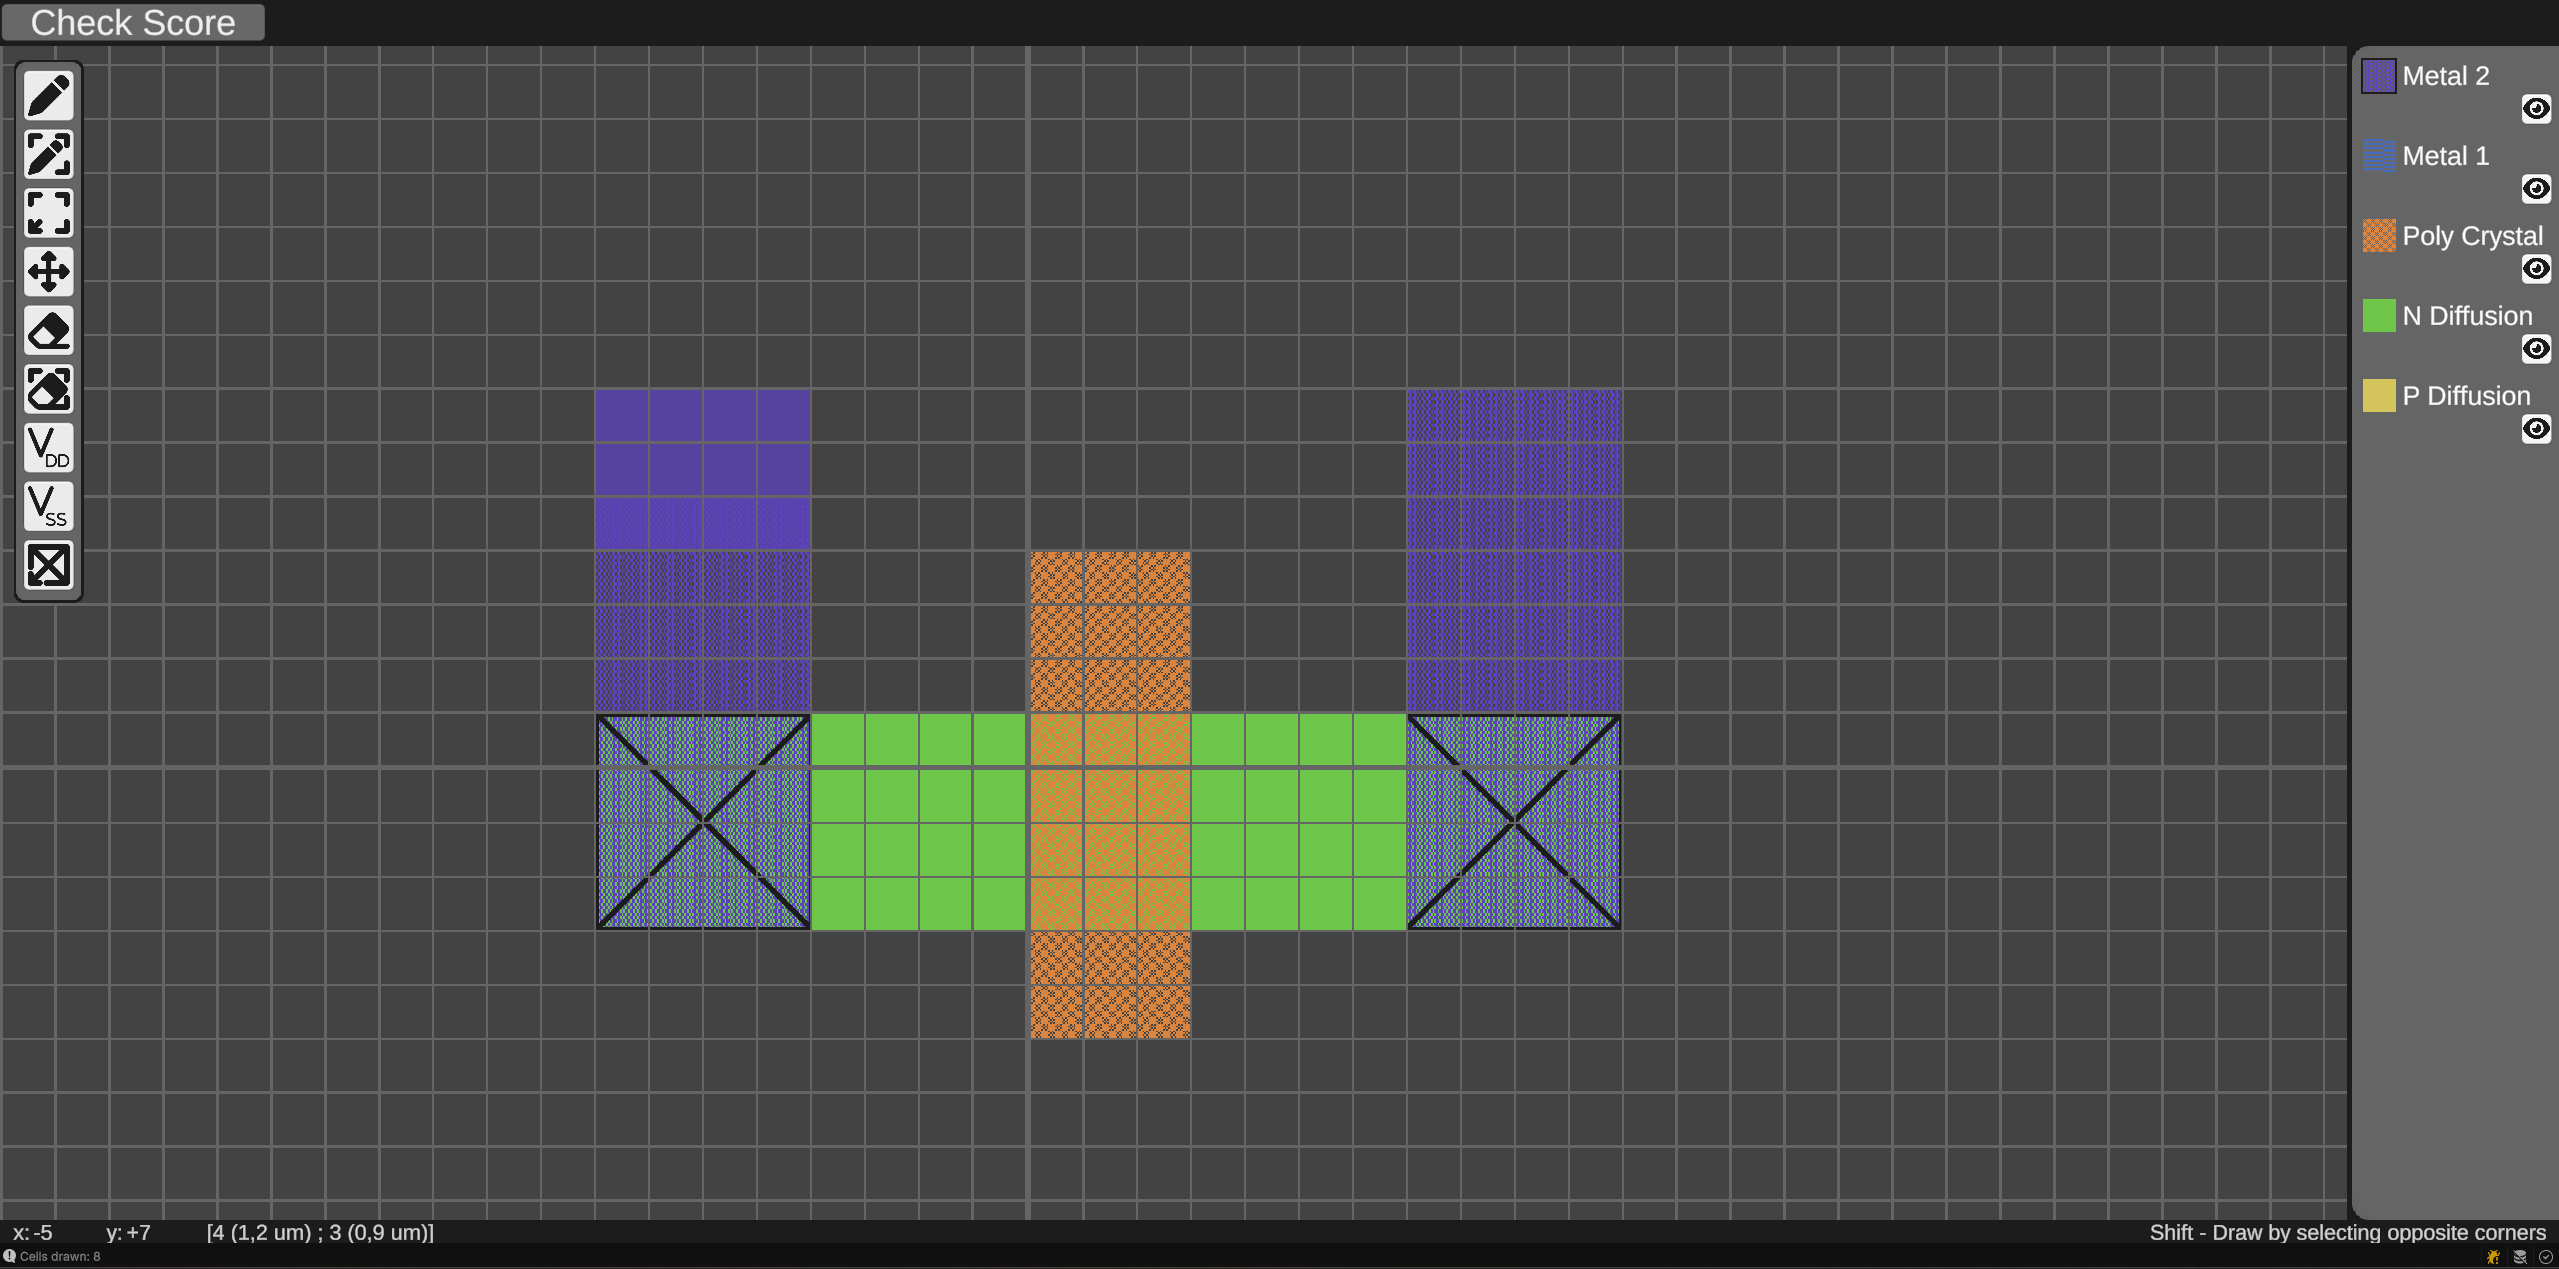
\includegraphics[width=0.9\textwidth]{chapters/chapter4/rys/final_ui}
    \caption[Widok okna aplikacji podczas pracy.]
    {Widok okna aplikacji podczas pracy, źródło: opracowanie własne.}
    \label{fig:ui_final}
\end{figure}

Z prawej strony znajduje się panel warstw, który umożliwia wybór warstwy, którą użytkownik chce rysować.
Każda z nich jest reprezentowana przez przycisk, który pozwala na jej wybór,
jej nazwę oraz dodatkowy przycisk do wyłączenia widoczności warstwy.
Panel taki dla każdej z warstw jest generowany dynamicznie na podstawie konfiguracji warstw \texttt{LayerConfig},
pobrany z menedżera warstw, \texttt{LayersManager}.
Na tej podstawie ustawiana jest nazwa warstwy oraz tekstura\linebreak i kolor w przycisku wyboru.\\
%\indent Panel narzędzi znajduje się po lewej stronie okna.
%W przeciwieństwie do warstw, przyciski do wyboru narzędzia są konfigurowane w edytorze Unity,
%poprzez przypisanie im \texttt{ToolConfig}.
%To z niego pobierane są informacje o ikonie narzędzia, podpowiedzi, jaka się wyświetli po najechaniu na przycisk
%oraz przypisany do narzędzi klawisz skrótu.\\
Panel narzędzi znajduje się po lewej stronie okna.
W przeciwieństwie do warstw, przyciski wyboru narzędzia konfiguruje się w edytorze Unity,
przypisując im \texttt{ToolConfig}.
Z niego pobierane są informacje o ikonie,
podpowiedzi wyświetlanej po najechaniu na przycisk oraz przypisanym klawiszu skrótu.\\
\indent W dolnej części okna znajduje się pasek informacyjny.
%Znajduje się tam wskaźnik aktualnej pozycji kursora na siatce, a także dodatkowe informacje o narzędziu,
%takie jak klawisze modyfikujące działanie oraz komunikaty, jakie może te narzędzie przekazywać.
%Gdy wybrane jest narzędzie obszarowe,
%wyświetlana są dodatkowo wymiary zaznaczonego obszaru na siatce oraz wymiary przemnożone przez parametr $\lambda$.
%W przypadku korzystania z narzędzia przesuwania podawane są informacje o przemieszczeniu w osiach $x$ i $y$.
Panel zawiera wskaźnik aktualnej pozycji kursora na siatce oraz dodatkowe informacje o narzędziu,
takie jak klawisze modyfikujące jego działanie i przekazywane przez niego komunikaty.
W przypadku wybrania narzędzia obszarowego wyświetlane są wymiary zaznaczonego obszaru na siatce
oraz ich wartości przeliczone z uwzględnieniem parametru $\lambda$.
Przy korzystaniu z narzędzia przesuwania podawane są natomiast informacje\linebreak o przemieszczeniu w osiach $x$ i $y$.
